\chapter{Literature Review}

This chapter presents the background theory for which this thesis is based upon.

\todo{improve introduction to chapter...}






\section{Network Delay and Latency}

The time it takes for a bit of data to travel across the network from one communication endpoint to another is known as \textit{delay}. The process for such a transmission involves many components. A typical example where the data traverses an intermediate device before reaching destination follows. First, the data to be sent is usually created by an application. The data will then be handed over to the \gls{os} which passes it further down to the network interface card. From there, the data will be encoded and transmitted over a physical medium and eventually received by an intermediate device, such as a router. The router will then analyze the data and retransmit it over another medium that points to the destination. Finally, the data reaches the receiver. The whole process can happen in either multiples or fractions of seconds.

\todo{maybe show a picture of the typical example}

Network delay is therefore divided into the following four parts:

\begin{itemize}
    \item Processing delay --- time it takes a router to process the packet header
    \item Queuing delay --- time the packet spends in routing queues
    \item Transmission delay --- time it takes to push the packet's bits onto the link
    \item Propagation delay --- time for a signal to reach its destination
\end{itemize}

It is common to notify the sender that the receiver actually got the data. This is done by sending a signal from the receiver back to the sender, known as an \gls{ack}. The total time it takes for a sender to send data \textit{and} receive back an \gls{ack} is known as \textit{latency} or \gls{rtt}.

In this thesis, we are mainly concerned with the \textit{queuing} delay part.

% \section{Bufferbloat}

% A common cause of latency in packet switched networks is bufferbloat. It occurs when a router, with a large buffer gets congested. the tcp \gls{cc} will fill up the entire buffer, before it starts backing off. Packets become queued for a long period of time, untill the buffer is drained, \gls{cc} resets and TCP connection ramps back up to speed to fill the buffer again.

% This causes high and variable latency, in addition to "blocking" the bottleneck for other flows when the buffer is full and packets are droped. Several technical solutions exists, that try to solve the problem of bufferbloat and we will outline some of them  in this section.









\section{Transmission Control Protocol}

Whenever a user sends an email, or any data over the network for that matter, one should expect some kind of assurance that the delivery of the data was successful. This notion is known as \textit{reliability}, and is one of the key components of the \gls{tcp} and why it is one of the main protocols for transmitting data on the Internet. In essence, \gls{tcp} is a communication protocol that provides reliable, ordered, and error-checked delivery of data between applications such as \gls{www}, email and file transfer.

\todo{write a bit more about tcp in general such a connection management and flow control}

% Today, most online web services \todo{citation} are based on transmissions from the \gls{tcp}.
\subsection{Reliability}
To ensure reliability, every tcp segment contains a sequence number, and an ACK is send back to the 
sender for every segment that is recived. This way, data that come out of order can be reordered on the 
reciving end. This also ensures that lost packets can be retransmitted. If one segment in a datastream is
lost, the reciver will only ACK the last \textit{in order} packet. Say segment nr 10 is lost. On receiving nr 11, the receiver
will ACK nr 9 again, this is called duplicate acknowledgment(DupAcks), and on receiving three DupAcks the sender will 
retransmitt the lost packet. A threshold of three is used in case the segment was just reordered by the network, to
avoid unnecessary retransmission.
Loss can also be detected by Retransmission timeout (RTO). For every segment that is sent a timer is started with 
an estimate of the arrival of the ACK. If the timer expires the segment is retransmitted and a new timer is started
with double length. This is to backoff retransmission trafic in case of malicious actors such as denial of service
attacks.

\subsection{Flow Controll}
Tcp stores the data to send in a send buffer before it goes out on the network, and the data it receives in a 
receive buffer before it is prosessed by an application. It is important to not send more data when the receive 
buffer is full, otherwise it would lead to packet drop. Tcp ensures this by maintaining a receive window and 
advertising it in every ACK. The receive window is the space left in the receive buffer, and it dictates how many 
unacknowledged packets can be in fligh at a time. This means that if the reciver is processing slowly, the receive 
buffer will start to fill up, causing the recevie window to to decrease, wich tells the sender to slow down
its sending rate.

% \gls{tcp} is the one of the main protocols for transmitting data on the internet. It is a connection based, reliable protocoll and is used by for instance World Wide Web (WWW), email, File Transfer Protocoll (FTP) and streaming media. \gls{tcp} requires that the sender and reciever establishes a connection through a three-way handshake before transmission starts. All segments sent have a sequence number, and the reciver sends an \gls{ack} for every segment it recieves. This, in addition to retransmission and error-checking ensures reliable transfer, but also lengthens latency.

\subsection{Network Congestion}

In the same sense that traffic on the road can come to a halt, the same is true for traffic on a network. This is known as \textit{congestion}, and is usually caused by overutilization. That is, network devices such as a router have finite resources, and thus too much traffic will cause the device to carry more data than it can handle which leads to congestion on the network. Typical effects include queueing delay, packet loss or the blocking of new connections.

\todo{show image illustrating congestion}

\todo{write more about general network congestion...}





\subsection{Congestion Control}

Another key compononent of \gls{tcp} is the ability to either prevent congestion or mitigate it after it occurs, known simply as \gls{cc}. The means of applying \gls{cc} is simple --- ensure that the sender does not overflow the network. In other words, the sender's rate needs to be adjusted based on the condition of the network. Now to the hard part --- how to adjust it?

To shed some light on this, \gls{tcp} includes a state variable called \gls{cwnd} which limits the amount of data that a sender can send before receiving an \gls{ack} back. This variable is known only to the sender, and serves as the key role for attaining \gls{cc}. The means of adjusting \gls{cwnd} is referred to as an \textit{congestion-control algorithm}, and consists of four intertwined parts:

\begin{itemize}
    \item Slow start ---
    \item Congestion avoidance ---
    \item Fast retransmit ---
    \item Fast recovery ---
\end{itemize}

The following sections will describe each part in more detail.




\subsubsection{Slow Start and Congestion Avoidance}

% Upon a \gls{tcp} connection, the value of \gls{cwnd} is typically set to a small multiple of the \gls{mss} allowed \cite{rfc6691}. The sending rate can then be calculated as follows:

% \begin{equation}
%     RATE = \frac{CWND}{RTT}.    \label{eq:rate}
% \end{equation}

% \begin{wrapfigure}{r}{0.35\textwidth}
%     \centering
%     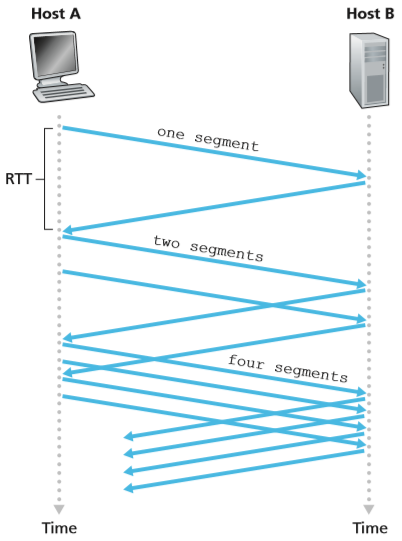
\includegraphics[width=0.35\textwidth]{TCP_Slow_Start}
%     \captionsetup{width=0.35\textwidth}
%     \caption{\gls{tcp} slow start.}
% \end{wrapfigure}

% With the initial \gls{cwnd} size set, say $1$ \gls{mss} for simplicity sake, the goal of the slow start phase is simple; find the amount of available bandwidth, \textit{quickly}.

% To do this, \gls{tcp} will first send one segment of size $1$ \gls{mss} into the network, and for every \gls{ack}, increase 

Slow start and congestion avoidance are two independent algorithms with
different objectives, but in practice are implemented together and so will be discussed together.

Upon a \gls{tcp} connection, the \gls{cwnd} value is initialized to a single \textit{segment} with a specified size. This size is either  announced by the the other end, known as the \gls{rwnd}, or set to a typical default \cite{rfc5681}. In the same sense that \gls{cwnd} is a sender-side limit, \gls{rwnd} is a receiver-side limit. Together, the minimum of \gls{cwnd} and \gls{rwnd} governs the data transmission in slow start. However, at the beginning of a transmission, the network conditions are unknown, so the goal of the slow start phase is simple --- slowly probe the network to determine the available capacity.

To find the capacity, slow start works as follows --- the sender starts by transmitting one segment. For every received \gls{ack}, increment the \gls{cwnd} by another segment, effectively doubling it every \gls{rtt}. Repeat this process until a timeout occurs. That is, until the capacity has been reached that is signaled by a router starting to drop packets, which tells the sender that its \gls{cwnd} has grown too large.

\begin{figure}[H]
    \centering
    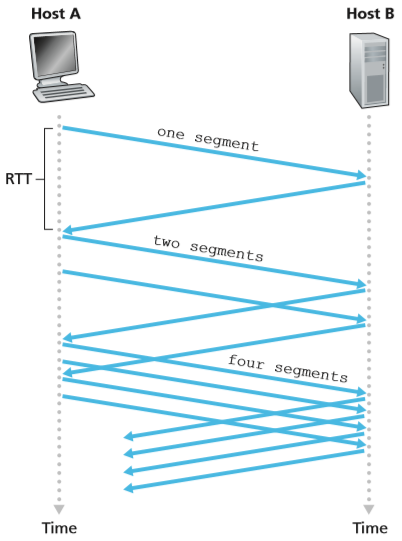
\includegraphics[width=0.4\textwidth]{TCP_Slow_Start}
    \captionsetup{width=0.4\textwidth}
    \caption{\gls{tcp} slow start. Despite the name, the sending rate experiences exponential growth. \todo{update image}}
\end{figure}

As a response to hitting the threshold, \gls{tcp} will now halve the \gls{cwnd} since that is the last known value to not induce a timeout. This new value is known as the \gls{ssthresh}, and is another \gls{tcp} state variable used to determine whether the slow start or congestion avoidance algorithm is used to control the data transmission. In other words, the slow start phase ends when \gls{cwnd} reaches or exceeds \gls{ssthresh}.

The goal of congestion avoidance is also simple --- avoid congestion, as the name implies. But the challenge here is to maintain a transmission rate that it not too low, otherwise the link becomes underutilized, and at the same time probe for available bandwidth without overflowing the network too quickly. To do so, a feedback control algorithm known as \gls{aimd} is used. \gls{aimd} provides linear growth of the \gls{cwnd} when probing for available bandwidth, and a multiplicative reduction when congestion is detected.

\begin{figure}[H]
    \centering
    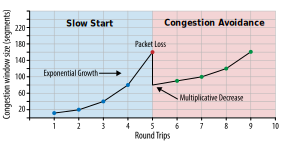
\includegraphics[width=0.7\textwidth]{TCP_Congestion_Control_Simple}
    \captionsetup{width=0.7\textwidth}
    \caption{The two main parts of \gls{cc} --- the slow start phase where \gls{cwnd} grows exponentially, and the congestion avoidance phase where the transmission rate is increased more conservatively. (\href{https://hpbn.co/building-blocks-of-tcp/}{\textit{source}})}
\end{figure}

\todo{maybe write more about AIMD with some math}

\todo{add conclusion to this section}




\subsubsection{Fast Retransmit and Fast Recovery}

Fast retransmit and fast recovery are two algorithms that aims to speed up the recovery process of a \gls{tcp} connection in the event of a segment loss, but without re-entering the slow start phase. As with slow start and congestion avoidance, both are in practice implemented together and so will be discussed together.

In a \gls{tcp} connection, the sender uses a simple timer to recognize lost segments. That is, if an \gls{ack} is not received within a specified time, the sender will assume that the segment has been lost and so will retransmit it. Fast retransmit is an enhancement to \gls{tcp} that reduces the time a sender waits before retransmitting a lost segment. The duration is determined by the amount of duplicate \gls{ack}s, which the receiver will keep sending to indicate the next expected sequence number. Generally, if only one or two duplicate \gls{ack}s are experienced, it is assumed that a simple reordering of the segments will solve the problem. But when three or more duplicate \gls{ack}s are received in a row, it signals a strong indication that a segment has been lost. In such a case, \gls{tcp} will perform a retransmission instead of waiting for a timeout, known as a \textit{fast transmit}.

When a fast retransmit has occured, the sender will transmit what appears to be the missing segment. However, the slow start phase will not be performed after this, but rather the congestion avoidance phase. This is known as the \textit{fast recovery} algorithm. Since only a segment seems to be missing, it would be wasteful to redue the traffic flow abruptly by going into slow start. Instead, a fast recovery is initiated, allowing for sustained high throughput under moderate congestion.

\begin{figure}[H]
    \centering
    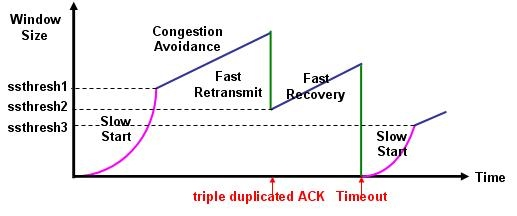
\includegraphics[width=0.6\textwidth]{TCP_Congestion_Control_Complete}
    \captionsetup{width=0.6\textwidth}
    \caption{A more complete illustration of a congestion-control algorithm including all four parts --- slow start, congestion avoidance, fast retransmit and fast recovery. \todo{update image}}
\end{figure}





% \subsubsection{Congestion Avoidance}
% \subsubsection{Fast Retransmit}
% \subsubsection{Fast Recovery}




% The answer is simple; \textit{start slow}. First, set the \gls{cwnd} to a small multiple of the \gls{mss} allowed on the \gls{tcp} connection. Then, start probing for available bandwidth. For every received \gls{ack}, double the \gls{cwnd} until a timeout occurs. This phase is known as the \textit{slow start}, which lasts until \gls{cwnd} reaches the threshold value, known as the \gls{ssthresh}, and is signaled by a timeout.

% With the threshold hit, \gls{tcp} now has an idea of the maximum amount of data it can transmit, and therefore sets the \gls{cwnd} value to half of the \gls{ssthresh} value since that is the last known value to not induce a timeout. From this point, the \textit{congestion avoidance} phase starts. Here, the \gls{cwnd} value is additively increased by one \gls{mss} every \gls{rtt}.





% \begin{figure}[H]
%     \centering
%     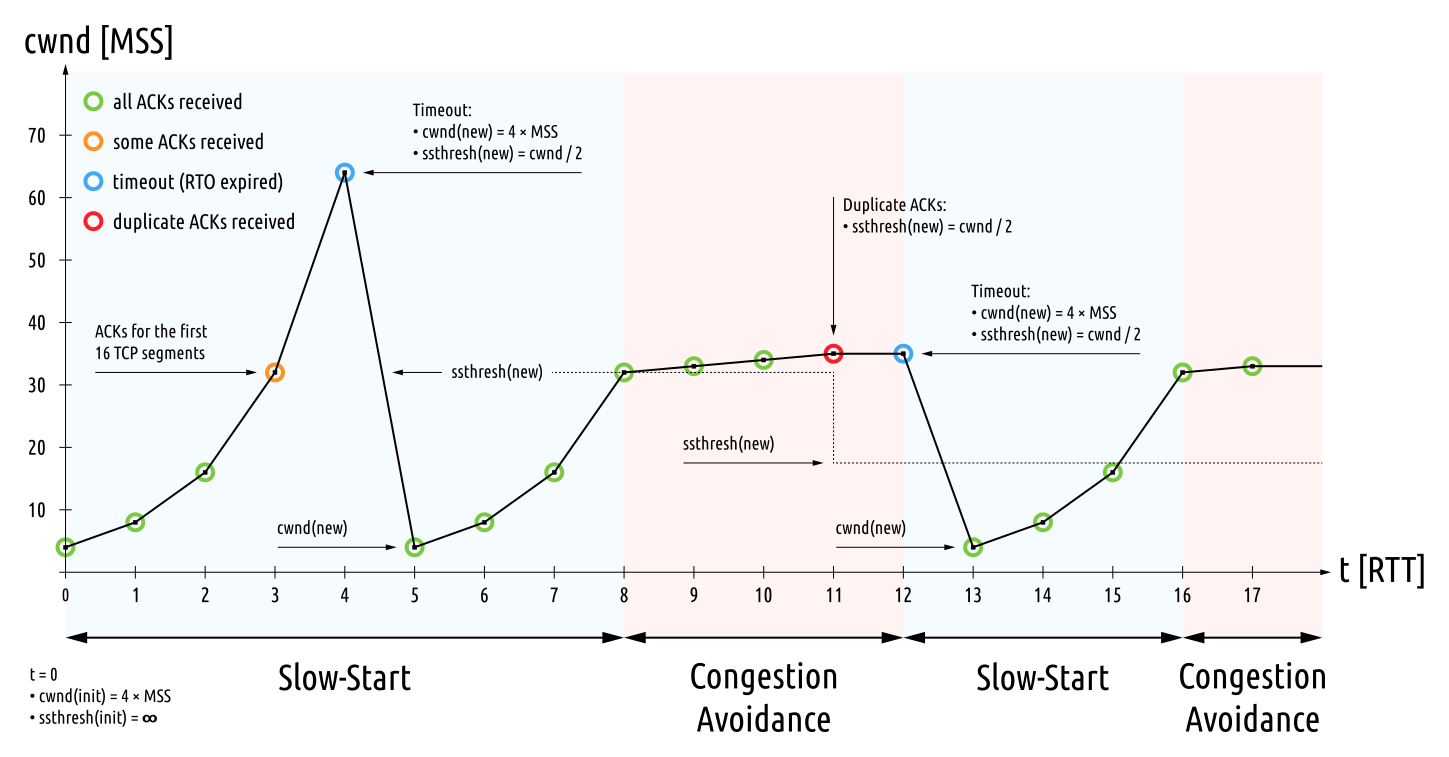
\includegraphics[width=1.0\textwidth]{TCP_Slow-Start_and_Congestion_Avoidance}
%     \captionsetup{width=0.95\textwidth}
%     \caption{Example of ioj oij io iojio joiojioj iojio joi jio joi jioj ioj io jio jioj ioj io jio ijojiojoijoij a parametric plot ($\sin (x), \cos(x), x$)}
% \end{figure}



% To help reduce congestion on the links \gls{tcp} maintains a \gls{cwnd}, which limits the total number of unacknowledged packets that it can send at a time. This is done in multiple fases.

% In the slow start fase,  right after a connection is established. the congestion window starts as a small multiple of \gls{mss} and is effectively doubled for every \gls{rtt}. When it reaches the slow-start threshold(ssthresh), \gls{cwnd} is reduced by half and a new fase starts, congestion avoidance. In this fase \gls{cwnd} is increased linearly by one \gls{mss} every \gls{rtt}. If loss occurs, it could mean there is congestion, and steps will be taken to reduce load on the network. The steps depend on what exact congestion avoidance algorithm is used.




\subsection{Bufferbloat}

It is easy to fall into the trap of believing that bigger buffers would increase network performance. After all, why drop a packet when you can avoid it by a buffer that never gets full in the first place. Likewise, it is easy to see why a big buffer is bad --- it takes time to drain the queue. If more packets come in than can be transmitted, the longer the queue gets. As a result, the latency spikes. Excess buffering of packets is referred to as \textit{bufferbloat}, causing high latency and reducing the overall network throughput.

Still, some buffering is clearly needed so that a short burst of packets can be absorbed without significant loss. But how much? Ideally, for a particular network, we would want to keep the bottleneck link as busy as possible. A widely used formula in determining the buffer size $B$ is the \gls{bdp}:

\begin{equation}
    B = RTT_{avg} \times C
\end{equation}

where $RTT_{avg}$ is the average \gls{rtt} of the flow passing through the link and $C$ is the capacity of the link. A well established rule of thumb is to provide $\SI{250}{\milli\second}$ or more for buffering. \cite{sizing_router_buffers} Say a router has a Gigabit Ethernet interface, then the buffer size should at least be $B = \SI{250}{\milli\second} \times \SI{1}{\giga\bit} = \SI{32}{\mega\byte}$.




\subsection{TCP Variants}

\todo{reno and tahoe, newreno, cubic, vegas, westwood, bbr etc.. A collection of brief explanations.}

\begin{figure}[H]
    \centering
    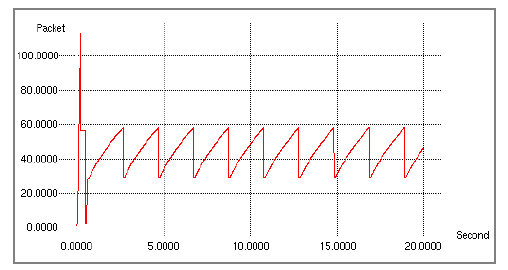
\includegraphics[width=0.6\textwidth]{TCP_CC_NewReno}
    \captionsetup{width=0.6\textwidth}
    \caption{The classic \textit{sawtooth} pattern of \gls{cwnd} using the \gls{tcp} congestion-algorithm known as \textit{NewReno}. \todo{update image}}
\end{figure}








\section{Active Queue Management}

When a packet arrives at the incoming port of a router, it is often the case that there is not enough memory to buffer it, and so an important decision must be made --- should the newly arrived packet simply be dropped, or should one of the already-queued packets be dropped to make room for the new one? In the early days of networking, the queue management algorithm called \textit{tail drop} was used, simply dropping newly arrived packets when the queue was filled. However, this approach is considered unfair among traffic flow due to its \textit{first come, first serve} basis, leaving little room for new participants since a single connection could monopolize the queue space. \cite{on_traffic_phase_effects_in_packet_switched_gateways} Tail drop also lead to what is known as \textit{\gls{tcp} global synchronization}, where all connections would both simultaneously "hold back" and then step forward, causing networks to become underutilized and flooded in alternate waves.

Over the years, many new suggestions and algorithms were made. They collectively became known as \gls{aqm} algorithms --- the policy of how to queue new incoming packets \textit{before} a buffer becomes full. One of the first and most widely implemented algorithm to surface was \gls{red}, addressing the issues of tail drop. By preemptively dropping packets \textit{probabilistically} before the buffer became full, \gls{red} would avoid both global synchronization and the problem of new bursty connections being penalized. \cite{ieee251892}

Widespread usage of \gls{red} also revealed a core problem --- it was difficult to configure, requiring complex fine-tuning in order to achieve significant performance gains. Variants of \gls{red} were developed to accommodate for this, such as BLUE, and later many new \gls{aqm} schemes. A few selected will be discussed briefly in the next sections.



\subsection{Controlled Delay}

\gls{codel} is a more recent \gls{aqm} scheme developed by Van Jacobsen. It is designed to overcome bufferbloat in modern networking environments by limiting, or \textit{controlling}, the delay that network packets experience when passed through buffers in networking hardware. An implementation of \gls{codel} for the Linux kernel was written in 2012 by Dave Täht and Eric Dumazet. It has since been adopted as the standard \gls{aqm} for the widely known OpenWrt \gls{os} used by many routers.

Van Jacobsen himself asserted in 2006 that existing \gls{aqm}s have been using incorrect means of recognizing bufferbloat. \cite{a_rant_on_queues} Algorithms such as \gls{red} measures the average queue length and considers it a case of bufferbloat if the average grows too large. Jacobsen demonstrated in 2006 that this is not necessarily the case, as a quick burst also exhibits the same behaviour. In fact, Jacobsen would say that queue length was no indicator at all about packet demand or network load, \cite{a_rant_on_queues, controlling_queue_delay} suggesting instead that the minimum queue length during a sliding time window would be a better metric. \cite{controlling_queue_delay}

Jacobsen would therefore properly combat bufferfloat in \gls{codel} by distinguishing between two types of queue --- a \textit{good} queue that exhibits no bufferbloat, and a \textit{bad} queue that actually exhibits bufferbloat. The \gls{codel} approach, in summary, is designed to meet the following goals: \cite{rfc8289}

\begin{itemize}
    \item Make \gls{aqm} parameterless for normal operation.
    \item Be able to distinguish a good queue from a bad one in order to keep delay low while allowing necessary bursts of traffic.
    \item Control delay while insensitive to \gls{rtt} delays, link rates, and traffic loads --- all without harming the network.
    \item Adapt to dynamically changing link rates with no negative impact on utilization.
    \item Allow simple and efficient implementation.
\end{itemize}

\todo{more details?}



\subsection{Proportional Integral Controller Enhanced}

\gls{pie} is another recent \gls{aqm} algorithm to control queuing latency directly in order to address the bufferbloat problem. It was made by a group of authors from Cisco Systems as a lightweight alternative to \gls{codel}, claiming that \gls{codel} cannot practically be implemented in hardware --- first, \gls{codel} requires packets to be timestamped when enqueued, and second, the drop decision happens on dequeue, so all packets have to be queued. \gls{pie}, on the other hand, performs the drop decision on enqueue, similar to \gls{red} and most other \gls{aqm} schemes. Hence, \gls{pie} incurs very little overhead and is simple enough to implement in both hardware and software.

The \gls{pie} approach, much like \gls{codel}, is designed to meet the following goals: \cite{rfc8033}

\begin{itemize}
    \item Control queuing latency instead of queue length to combat bufferbloat.
    \item Attaining a delicate balance between high link utilization and low latency.
    \item Simple to implement and easily scalable in both hardware and software by striving to maintain similarity to that of \gls{red}.
    \item Ensure system stability for various network topologies and scale well across an arbitrary number of streams.
    \item Design parameters should be set automatically. Users only need to set performance-related parameters such as target queue latency, not design parameters.
\end{itemize}







\section{Explicit Congestion Notification}

Conventially, the means of detecting network congestion has been by packet loss or a long enough delay inducing a timeout. Then the addition of \gls{aqm} came to the Internet infrastructure, adding the ability for routers to detect congestion before the queue overflows. Both loss and delay are \textit{implicit} signals of congestion, and in 2001, an extension to \gls{tcp} and \gls{ip} was defined \cite{rfc3168} to allow for \textit{explicit} congestion signaling --- called \gls{ecn} --- enabling end-to-end notification of network congestion without dropping packets.

\begin{wraptable}{r}{9cm}
    \begin{tabular}{|c|l|l|}
        \multicolumn{3}{c}{ECN Code Points} \\
        \hline
        Code & Description & Shorthand \\
        \hline
        00 & Non ECN-Capable Transport & Non-ECT \\
        \hline
        01 & ECN Capable Transport & ECT(0) \\
        \hline
        10 & ECN Capable Transport & ECT(1) \\
        \hline
        11 & Congestion Encountered & CE \\
        \hline
    \end{tabular}
    \caption{The four different code points for \gls{ecn} that is encoded in the \gls{ip} header.}
    \label{table:ecn}
\end{wraptable}

\gls{ecn} is a form of network-assisted \gls{cc}, meaning that the entire underlying network infrastructure must support it. For this to work, the new \gls{ecn} mechanism consists of two components:

\begin{itemize}
    \item Two new bits has been added to the \gls{ip} header in order to explicitly communicate \gls{ecn}-capability and indication of congestion on the network (see table \ref{table:ecn}).
    \item Two new flags has been added to the \gls{tcp} header --- the \gls{ece} flag so that the receiver can inform a sender when a \gls{ce} packet has been received, and the \gls{cwr} flag so that a sender can inform the receiver that the \gls{cwnd} has been reduced.
\end{itemize}

An \gls{ecn}-capable network works as follows. A sender will transmit \gls{ip} packets with either the \gls{ect}(0) or \gls{ect}(1) bit set. Then, when there is congestion, a router (in conjuction with \gls{aqm}) will start marking the packets by setting the \gls{ce} bit. The receiver will then see this, and echo back the congestion indication to the sender with an \gls{ece} packet. The sender will then reduce its \gls{cwnd} value and respond with an \gls{cwr} packet.

\todo{go on...}




% \subsection{Legacy ECN}

% In legacy ECN, the router notifies end hosts of congestion by setting a Congestion Encountered (CE) flag in the \gls{ip} header on ECN enabled packets when experiencing congestion. The receiver of the packet then reflects this back to the sender by setting an ECN-Echo (ECE) in the TCP header. It keeps doing this until the sender responds back with a segment with Congestion Window Reduced (CWR) set, indicating that the sender has backed off.




% \subsection{Accuracy ECN}





\section{Alternative Backoff with ECN}

The standard response to a packet loss in a \gls{tcp} connection is to reduce the \gls{cwnd} value by half, as with NewReno. \todo{go on...}